%%% CSE 4317 DDS - WORKED EXAMPLE (Mobile App + IoT). Follows IEEE Std 1016-2009.
\documentclass[11pt,letterpaper]{article}
\usepackage[margin=1.0in]{geometry}
\usepackage[T1]{fontenc}\usepackage[bitstream-charter]{mathdesign}\usepackage[latin1]{inputenc}
\usepackage{amsmath}\usepackage{xcolor}\usepackage{cite}\usepackage{hyphenat}
\usepackage{graphicx}\usepackage{float}\usepackage{subfigure}\usepackage{sectsty}
\usepackage[compact]{titlesec}\usepackage[tablegrid]{vhistory}\usepackage{pbox}\usepackage{longtable}
\usepackage{tikz}\usetikzlibrary{positioning,arrows.meta,fit,backgrounds}
\allsectionsfont{\color{accentcolor}\scshape\selectfont}
\definecolor{accentcolor}{rgb}{0.0,0.0,0.5}
\tikzset{
  mod/.style={draw, rounded corners, fill=white, minimum height=8mm, minimum width=27mm, font=\footnotesize, align=center, inner sep=2pt},
  ext/.style={draw, dashed, rounded corners, fill=black!4, minimum height=8mm, minimum width=24mm, font=\footnotesize\itshape, align=center, inner sep=2pt},
  band/.style={draw=accentcolor!45, rounded corners, inner sep=3.5mm},
  llbl/.style={font=\small\bfseries, text=accentcolor, align=left},
  flow/.style={-{Latex[length=2mm]}, thick, draw=accentcolor!80},
  fl/.style={font=\scriptsize, fill=white, inner sep=1pt},
}
\newcommand{\teamname}{Team Nimbus}
\newcommand{\productname}{AquaGuard Smart Water-Leak Monitor}
\newcommand{\coursename}{CSE 4317: Senior Design II}
\newcommand{\semester}{Spring 2027}
\newcommand{\docname}{Detailed Design Specification}
\newcommand{\department}{Department of Computer Science \& Engineering}
\newcommand{\university}{The University of Texas at Arlington}
\newcommand{\authors}{Alan Turing \\ Grace Hopper \\ John Von Neumann \\ Ada Lovelace \\ Charles Babbage}
\usepackage{fancyhdr}\pagestyle{fancy}\usepackage{lastpage}
\lhead{}\chead{}\rhead{}\lfoot{\footnotesize \teamname \ - \semester}\cfoot{}
\rfoot{\footnotesize page \thepage\ of \pageref{LastPage}}
\renewcommand{\headrulewidth}{0.0pt}\renewcommand{\footrulewidth}{0.4pt}
\usepackage[runin]{abstract}\abslabeldelim{\quad}\setlength{\abstitleskip}{-10pt}
\renewcommand{\abstractname}{}\renewcommand{\abstracttextfont}{\color{accentcolor} \small \slshape}

\begin{document}
{\centering \huge \color{accentcolor} \sc \textbf{\department \\ \university} \par}
\vspace{1 in}
{\centering \huge \color{accentcolor} \sc \textbf{\docname \\ \coursename \\ \semester} \par}
\vspace{0.5 in}
\begin{figure}[h!]\centering
\includegraphics[width=0.60\textwidth]{images/test_image}\end{figure}
\vspace{0.5 in}
{\centering \huge \color{accentcolor} \sc \textbf{\teamname \\ \productname} \par}
\vspace{0.5 in}{\centering \large \sc \textbf{\authors} \par}
\newpage
\begin{versionhistory}
  \vhEntry{0.1}{01.20.2027}{CB}{document creation}
  \vhEntry{1.0}{02.05.2027}{AT|GH|CB}{official release}
\end{versionhistory}
\newpage\setcounter{tocdepth}{2}\tableofcontents\newpage

\section{Introduction}
Implementation-level design of \productname\ as an IEEE 1016-2009 \cite{IEEE1016}
Software Design Description, building on the SRS and ADS (layers X/Y/Z).

\section{Design Stakeholders \& Concerns}
Firmware/app/cloud implementers, integrators, testers, support; concerns of
composition, data, interfaces, timing/state, algorithms, and resources.

\section{Design Viewpoints}
Context, Composition, Information, Interface, Interaction \& State, Algorithm,
Resource per IEEE 1016; omitted where not applicable.

\section{System Overview}
\begin{figure}[h!]\centering\resizebox{\textwidth}{!}{%
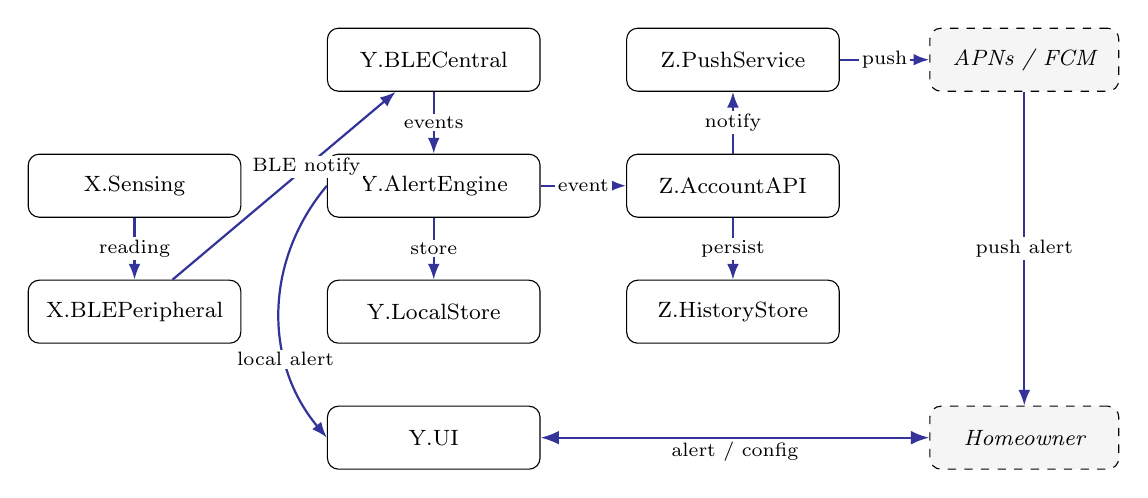
\begin{tikzpicture}
\node[mod] (xsens) at (2.6,0.8) {X.Sensing};
\node[mod] (xble)  at (2.6,-0.8){X.BLEPeripheral};
\node[mod] (ybc)  at (6.4,2.4) {Y.BLECentral};
\node[mod] (yae)  at (6.4,0.8) {Y.AlertEngine};
\node[mod] (yls)  at (6.4,-0.8){Y.LocalStore};
\node[mod] (yui)  at (6.4,-2.4){Y.UI};
\node[mod] (zpush) at (10.2,2.4){Z.PushService};
\node[mod] (zapi)  at (10.2,0.8){Z.AccountAPI};
\node[mod] (zhist) at (10.2,-0.8){Z.HistoryStore};
\node[ext] (apns) at (13.9,2.4){APNs / FCM};
\node[ext] (home) at (13.9,-2.4){Homeowner};
\draw[flow] (xsens) -- (xble) node[fl,pos=0.5]{reading};
\draw[flow] (xble) -- (ybc) node[fl,pos=0.6]{BLE notify};
\draw[flow] (ybc) -- (yae) node[fl,pos=0.5]{events};
\draw[flow] (yae) -- (yls) node[fl,pos=0.5]{store};
\draw[flow] (yae.west) to[bend right=40] node[fl,pos=0.68]{local alert} (yui.west);
\draw[flow] (yae) -- (zapi) node[fl,pos=0.5]{event};
\draw[flow] (zapi) -- (zpush) node[fl,pos=0.5]{notify};
\draw[flow] (zapi) -- (zhist) node[fl,pos=0.5]{persist};
\draw[flow] (zpush) -- (apns) node[fl,pos=0.5]{push};
\draw[flow] (apns) -- (home) node[fl,pos=0.5]{push alert};
\draw[{Latex}-{Latex}, thick, draw=accentcolor!80] (yui) -- (home) node[fl,pos=0.5,below]{alert / config};
\end{tikzpicture}}
\caption{Device/app/cloud architecture carried forward from the ADS}\end{figure}
Device: nRF52-class MCU with integrated BLE (C/Zephyr). App: Flutter (Dart) for
iOS/Android parity. Cloud: a small serverless API + managed DB + APNs/FCM.

\section{X Layer Subsystems --- Sensor Device}
\subsection{Layer Resources}
\textbf{Hardware:} nRF52 MCU + BLE, capacitive moisture pad, flow sensor, coin/AA
battery. \textbf{OS:} Zephyr RTOS. \textbf{Language:} C.
\subsection{X.Sensing}
\textbf{Information:} \texttt{Reading\{ts, moisture, flow, battery\_mV\}}.
\textbf{Algorithm:} periodic ADC sample; a debounced threshold with hysteresis
raises \texttt{leak=true} (FR-01); duty-cycled to meet PE-01. \textbf{State:}
\texttt{IDLE$\rightarrow$SAMPLING$\rightarrow$LEAK} with cooldown.
\subsection{X.BLEPeripheral}
\textbf{Interface (\#01, GATT):} \texttt{svc AquaGuard}: char \texttt{reading}
(notify), \texttt{leak} (notify), \texttt{threshold} (read/write), \texttt{battery}
(read). \textbf{Interaction:} bonded, encrypted connections only (SE-01); advertises
when idle. \textbf{Rationale:} standard GATT keeps the app contract simple (AD-01).

\section{Y Layer Subsystems --- Mobile Application}
\subsection{Layer Resources}
\textbf{Deps:} Flutter, a BLE plugin, a push plugin, local DB (SQLite);
\textbf{Language:} Dart. \textbf{Platforms:} iOS + Android (QA-01).
\subsection{Y.BLECentral}
\textbf{Interface (\#02):} scan/connect/bond; subscribe \texttt{reading}/\texttt{leak};
write \texttt{threshold}. \textbf{State:}
\texttt{DISCONNECTED$\rightarrow$SCANNING$\rightarrow$CONNECTED$\rightarrow$BONDED}
with auto-reconnect. \textbf{Rationale:} platform BLE-background differences isolated
here so the rest of the app is platform-agnostic (QA-01).
\subsection{Y.AlertEngine, Y.UI, Y.LocalStore}
\textbf{Y.AlertEngine:} on \texttt{leak} while connected, fire local
notification/haptic within 3\,s (FR-03); if disconnected, POST the event to the
backend for push (FR-04). \textbf{Y.UI:} guided setup wizard, live status, and
history list (US-01, FR-05). \textbf{Y.LocalStore:} SQLite
\texttt{events\{ts, type, value\}} and \texttt{config}.

\section{Z Layer Subsystems --- Cloud Services}
\subsection{Layer Resources}
\textbf{Tech:} serverless functions + managed DB; \textbf{Language:} TypeScript.
\subsection{Z.AccountAPI \& Z.HistoryStore}
\textbf{Interface:} \texttt{POST /events}, \texttt{GET /events}, device/user
registration over TLS 1.3 (SE-01). \textbf{Information:}
\texttt{Event\{device\_id, ts, type, value\}} in the managed DB (FR-05).
\subsection{Z.PushService}
On event ingest, look up the user's device token and send via APNs/FCM (EI-02,
FR-04); delivery failures retried and logged (MS-01).

\section{Requirements Traceability}
\begin{table}[H]\begin{center}\begin{tabular}{ | p{1.6cm} | p{5cm} | p{3.4cm} | p{1.6cm} |}\hline
\textbf{Req} & \textbf{Requirement (abbrev.)} & \textbf{Component} & \textbf{Iface} \\ \hline
FR-01 & Leak detection & X.Sensing & \#01 \\ \hline
FR-02 & Pair/config & Y.BLECentral, X.BLEPeripheral & \#02/\#01 \\ \hline
FR-03 & Local alert & Y.AlertEngine & --- \\ \hline
FR-04 & Remote alert & Z.PushService & --- \\ \hline
FR-05 & History & Y.LocalStore, Z.HistoryStore & --- \\ \hline
SE-01 & Secure pair/TLS & X.BLEPeripheral, Z.AccountAPI & \#01 \\ \hline
\end{tabular}\end{center}\end{table}

\section{Appendix A}
BLE GATT profile table, firmware power budget, enclosure CAD (STEP), and wiring
schematic are attached to the closeout package.

\bibliographystyle{reference/IEEEtran_custom}
\bibliography{reference/refs}{}
\end{document}
